\documentclass[11pt,a4paper]{article}

% Custom packages and styling
\usepackage[utf8]{inputenc}
\usepackage[margin=1in]{geometry}
\usepackage{xcolor}
\usepackage{hyperref}
\usepackage{booktabs}
\usepackage{tabularx}
\usepackage{listings}
\usepackage{graphicx}
\usepackage{amsmath}
\usepackage{amssymb}
\usepackage{fancyhdr}
\usepackage{titlesec}
\usepackage{tikz}
\usetikzlibrary{shapes.geometric, arrows, positioning}
\usepackage{parskip} % Removes paragraph indent, adds spacing between paragraphs

% Custom color palette
\definecolor{primary}{HTML}{1A365D}   % Deep Navy
\definecolor{secondary}{HTML}{2B6CB0} % Bright Blue
\definecolor{accent}{HTML}{E2E8F0}    % Slate Gray
\definecolor{darkgray}{HTML}{2D3748}  % Charcoal
\definecolor{codebg}{HTML}{F7FAFC}    % Light Gray for code blocks
\definecolor{success}{HTML}{2F855A}   % Muted Green
\definecolor{warning}{HTML}{C05621}   % Muted Orange
\definecolor{danger}{HTML}{9B2C2C}    % Muted Red

% Setup hyperref
\hypersetup{
    colorlinks=true,
    linkcolor=primary,
    filecolor=secondary,      
    urlcolor=secondary,
    citecolor=primary,
    pdfauthor={Ali Shayan},
    pdftitle={AQI Predictor Report - Islamabad}
}

% Code snippet styling
\lstset{
    backgroundcolor=\color{codebg},
    basicstyle=\ttfamily\small\color{darkgray},
    breakatwhitespace=false,
    breaklines=true,
    captionpos=b,
    commentstyle=\color{gray},
    frame=single,
    keepspaces=true,
    keywordstyle=\color{secondary},
    numbers=left,
    numberstyle=\tiny\color{gray},
    rulecolor=\color{accent},
    showspaces=false,
    showstringspaces=false,
    showtabs=false,
    tabsize=2
}

% Header and Footer setup
\pagestyle{fancy}
\fancyhf{}
\fancyhead[L]{\textcolor{gray}{\small AQI Forecasting System for Islamabad}}
\fancyhead[R]{\textcolor{gray}{\small June 2026}}
\fancyfoot[C]{\textcolor{gray}{\small Page \thepage}}
\renewcommand{\headrulewidth}{0.5pt}
\renewcommand{\footrulewidth}{0pt}

% Section formatting
\titleformat{\section}
  {\color{primary}\normalfont\Large\bfseries}
  {\thesection}{1em}{}[{\color{secondary}\titlerule[1pt]}]
  
\titleformat{\subsection}
  {\color{secondary}\normalfont\large\bfseries}
  {\thesubsection}{1em}{}

\begin{document}

% Title Page
\begin{titlepage}
    \centering
    \vspace*{2cm}
    
    \Huge
    \textbf{\textcolor{primary}{Air Quality Index (AQI) Forecasting System for Islamabad, Pakistan}}
    
    \vspace{0.5cm}
    \LARGE
    \textcolor{secondary}{A Production-Grade MLOps System Report}
    
    \vspace{2cm}
    
    \makebox[\textwidth]{\color{secondary}\rule{\textwidth}{2pt}}
    
    \vspace{2cm}
    
    \large
    \begin{tabular}{ll}
        \textbf{Author:} & Ali Shayan \\
        \textbf{Organization:} & 10Pearls University --- Internship Program \\
        \textbf{Date:} & June 2026 \\
        \textbf{Version:} & 1.0
    \end{tabular}
    
    \vfill
    
    \makebox[\textwidth]{\color{accent}\rule{\textwidth}{1pt}}
    
    \vspace{0.8cm}
    \small
    \textbf{Live Dashboard:} \url{https://aqi-predictor.onrender.com} \\
    \textbf{GitHub Repository:} \url{https://github.com/iamalishayan/Pearls-AQI-Predictor}
    
    \vspace*{1cm}
\end{titlepage}

\newpage
\tableofcontents
\newpage

\section{Project Overview \& Objectives}

The goal of this project was to build a production-grade, end-to-end Air Quality Index (AQI) forecasting system for Islamabad, Pakistan. Air pollution is a critical public health concern in South Asian cities, and accurate short-term forecasts can help citizens and authorities make informed decisions about outdoor activities, school closures, and health advisories.

\subsection{Objectives}
\begin{itemize}
    \item \textbf{Predict $\text{PM}_{2.5}$ concentration} (the most harmful fine particulate matter) over a 3-day forecast horizon (+24h, +48h, +72h).
    \item \textbf{Train multiple ML models} (Ridge Regression, Random Forest, XGBoost) and automatically select the best performer per horizon using rigorous cross-validation.
    \item \textbf{Experiment with deep learning} (LSTM, GRU) to compare against traditional ensemble methods and document findings.
    \item \textbf{Deploy a fully automated MLOps pipeline} where new data is ingested hourly, models are retrained daily, and predictions are served via a live web dashboard.
    \item \textbf{Provide SHAP-based explainability} so users can understand \textit{why} the model predicts a specific AQI, not just \textit{what} it predicts.
    \item \textbf{Implement health alerts} that dynamically fire when predicted AQI crosses EPA-defined hazardous thresholds.
\end{itemize}

\subsection{Key Principles}
\begin{itemize}
    \item \textbf{No local data storage:} All features and models are stored in Hopsworks Feature Store and Model Registry --- the single source of truth.
    \item \textbf{Reproducibility:} Every training run is logged in MLflow with full hyperparameter and metric tracking.
    \item \textbf{Modularity:} The codebase is cleanly separated into independent pipelines (feature, backfill, training, inference) connected only through the Feature Store.
\end{itemize}

\newpage
\section{Architecture \& Design Decisions}

The system follows a modern \textbf{Serverless MLOps} architecture, built on a clear separation of concerns. The flowchart of data and training flow is illustrated in Figure \ref{fig:architecture}.

\begin{figure}[h!]
\centering
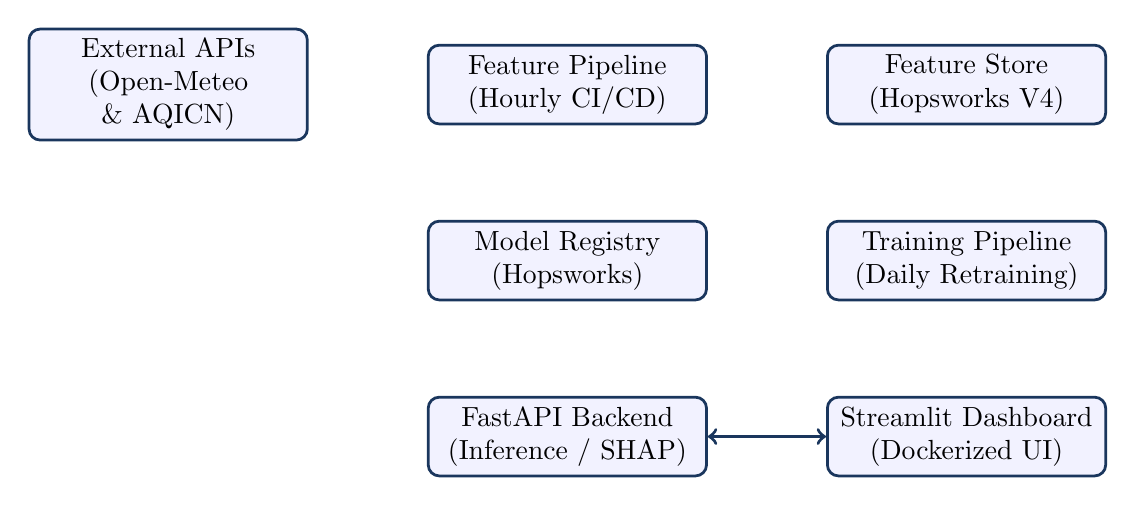
\begin{tikzpicture}[
    node distance=1.2cm and 1.5cm,
    block/.style={rectangle, draw, fill=blue!5, text width=3.3cm, text centered, rounded corners, minimum height=1cm, line width=1pt, draw=primary},
    arrow/.style={-stealth, line width=1.2pt, primary}
]
    % Nodes
    \node (apis) [block] {External APIs\\(Open-Meteo \& AQICN)};
    \node (feature) [block, right=of apis] {Feature Pipeline\\(Hourly CI/CD)};
    \node (store) [block, right=of feature] {Feature Store\\(Hopsworks V4)};
    \node (training) [block, below=of store] {Training Pipeline\\(Daily Retraining)};
    \node (registry) [block, left=of training] {Model Registry\\(Hopsworks)};
    \node (backend) [block, below=of registry] {FastAPI Backend\\(Inference / SHAP)};
    \node (frontend) [block, right=of backend] {Streamlit Dashboard\\(Dockerized UI)};
    
    % Paths
    \path [arrow] (apis) -- (feature);
    \path [arrow] (feature) -- (store);
    \path [arrow] (store) -- (training);
    \path [arrow] (training) -- (registry);
    \path [arrow] (registry) -- (backend);
    \path [arrow] (backend) -- (frontend);
    \draw [arrow, <->] (frontend.west) -- (backend.east); % Bidirectional communication
\end{tikzpicture}
\caption{Serverless MLOps System Architecture}
\label{fig:architecture}
\end{figure}

\subsection{Design Decisions}

\begin{table}[h!]
\centering
\small
\begin{tabularx}{\textwidth}{l X}
\toprule
\textbf{Decision} & \textbf{Rationale} \\
\midrule
\textbf{Hopsworks Feature Store} & Eliminates fragile local CSV files. Provides schema validation, versioning, and online/offline stores for both training and serving. \\
\addlinespace
\textbf{Separate Ingestion \& Retraining} & Decouples data ingestion from model training, allowing independent scaling, testing, and scheduling. \\
\addlinespace
\textbf{FastAPI + Streamlit} & FastAPI handles heavy inference computations and SHAP values, while Streamlit provides an interactive, responsive UI. \\
\addlinespace
\textbf{Docker Containerization} & Both services are containerized for environment parity, resolving local vs. production environment inconsistencies. \\
\addlinespace
\textbf{GitHub Actions CI/CD} & Hourly feature ingestion and daily model retraining are fully automated via cron-triggered workflows without needing dedicated servers. \\
\addlinespace
\textbf{SHAP explainability} & SHAP provides mathematically consistent Shapley values with native TreeExplainer support for our production models (Random Forest, XGBoost). \\
\bottomrule
\end{tabularx}
\caption{System Design Decisions and Rationale}
\label{tab:decisions}
\end{table}

\newpage
\section{Data Sources \& Preprocessing}

\subsection{Data Ingestion}
All data is sourced dynamically from \textbf{Open-Meteo's} free, open-source APIs, which provides historical and forecast weather and air pollution metrics:

\begin{table}[h!]
\centering
\small
\begin{tabularx}{\textwidth}{l l X}
\toprule
\textbf{API Source} & \textbf{Variables Collected} & \textbf{Purpose} \\
\midrule
Air Quality API & $\text{PM}_{2.5}$, $\text{PM}_{10}$, $\text{CO}$, $\text{NO}_2$, $\text{SO}_2$, $\text{O}_3$ & Target variable and pollutant features \\
Weather Archive API & Temp, Humidity, Pressure, Wind Speed, Precip & Meteorological drivers of pollution dispersion \\
AQICN API & Live AQI & Real-time validation comparison on the dashboard \\
\bottomrule
\end{tabularx}
\caption{Data Sources and Collected Variables}
\label{tab:data_sources}
\end{table}

\subsection{Preprocessing Steps}
\begin{enumerate}
    \item \textbf{Temporal Alignment:} Both weather and air quality data are fetched at hourly granularity, merged on exact timestamps, and sorted chronologically.
    \item \textbf{Missing Value Handling:} Forward-filling (\texttt{ffill}) is applied to handle any gaps in sensor readings, as atmospheric pollution levels change gradually.
    \item \textbf{Type Casting:} Integer columns (\texttt{hour}, \texttt{day\_of\_week}, \texttt{month}, \texttt{is\_weekend}, \texttt{is\_night}) are cast to \texttt{int32} for Hopsworks schema compatibility. Float columns are standardized to \texttt{float64}.
    \item \textbf{Timezone Normalization:} All timestamps are converted to UTC and then localized to naive datetimes for consistent Feature Store storage.
\end{enumerate}

\subsection{Backfill Pipeline}
Historical data spanning \textbf{90 days} (approximately 2,184 hourly rows) was ingested via a dedicated \texttt{backfill\_pipeline.py} script. This script fetches, engineers features, and uploads the historical dataset to Hopsworks Feature Group Version 4.

\section{Feature Engineering Methodology}

Feature engineering was the single most impactful step in improving model accuracy. Every engineered feature was mathematically justified through the EDA notebook.

\begin{table}[h!]
\centering
\small
\begin{tabularx}{\textwidth}{l l l X}
\toprule
\textbf{Feature} & \textbf{Type} & \textbf{Description} & \textbf{Justification} \\
\midrule
\texttt{hour} & Temporal & Hour of day (0--23) & Captures diurnal spikes (e.g. traffic \& night inversion) \\
\texttt{day\_of\_week} & Temporal & Day (0=Mon, 6=Sun) & Captures traffic variations by workday vs. weekend \\
\texttt{month} & Temporal & Month (1--12) & Captures seasonal pollution variations (e.g., winter smog) \\
\texttt{is\_weekend} & Binary & 1 if Saturday/Sunday & Reduced industrial/traffic emissions on weekends \\
\texttt{is\_night} & Binary & 1 if hour $\ge 20$ or $< 6$ & Atmospheric inversion traps pollutants at night \\
\texttt{pm25\_lag\_1h} & Lag & $\text{PM}_{2.5}$ value 1 hour ago & Short-term momentum of pollution levels \\
\texttt{pm25\_lag\_6h} & Lag & $\text{PM}_{2.5}$ value 6 hours ago & Medium-term trend tracking \\
\texttt{pm25\_lag\_24h} & Lag & $\text{PM}_{2.5}$ value 24 hours ago & Captures the dominant 24h autocorrelation cycle \\
\texttt{pm25\_change\_24h} & Delta & $\text{PM}_{2.5}$ current $-$ lag 24h & Captures rate of change (spikes vs. declines) \\
\texttt{pm25\_rolling\_mean\_24h} & Rolling & 24h rolling average & Smooths sensor noise and micro-fluctuations \\
\texttt{temp\_trend\_6h} & Trend & Temp change over 6 hours & Detects cold/warm fronts affecting inversion layers \\
\texttt{heat\_index} & Interaction & Temp $\times$ Humidity / 100 & Combined thermal stress indicator \\
\texttt{humidity\_wind\_interaction} & Interaction & Humidity $\times$ Wind Speed & Captures moisture-driven dispersion effects \\
\bottomrule
\end{tabularx}
\caption{Detailed Engineered Features (V4 Schema)}
\label{tab:features}
\end{table}

\subsection{Feature Store Versioning}
\begin{itemize}
    \item \textbf{V3:} Original feature set with lag features and rolling statistics.
    \item \textbf{V4 (current):} Added \texttt{pm25\_change\_24h} (AQI change-rate feature). The schema migration required creating a new Feature Group version and re-running the backfill pipeline.
\end{itemize}

\newpage
\section{Exploratory Data Analysis (EDA)}

A comprehensive EDA was performed in \texttt{notebooks/01\_eda.ipynb} to validate assumptions and guide feature engineering. Key findings include:

\subsection{Target Distribution}
$\text{PM}_{2.5}$ is \textbf{heavily right-skewed} with a long tail of extreme pollution events. This is typical for pollutant data and strongly favors tree-based models (Random Forest, XGBoost) over linear models, since tree-based algorithms are inherently robust to non-normal distributions.

\subsection{Temporal Patterns}
\begin{itemize}
    \item \textbf{Diurnal Cycle:} $\text{PM}_{2.5}$ peaks between 8--10 PM and again at 6--8 AM (rush hour + nighttime boundary layer collapse), confirming the importance of \texttt{hour} and \texttt{is\_night} features.
    \item \textbf{Weekend Effect:} Average $\text{PM}_{2.5}$ is measurably lower on weekends due to reduced industrial activity and traffic.
    \item \textbf{Seasonal Variation:} March-April shows higher pollution (pre-monsoon dry season), while June shows lower levels (monsoon washout).
\end{itemize}

\subsection{Feature Correlations}
\begin{itemize}
    \item \textbf{$\text{PM}_{10}$ and $\text{CO}$} are highly correlated with $\text{PM}_{2.5}$ ($\rho > 0.7$), as they share common combustion sources.
    \item \textbf{Wind speed} has a negative correlation ($\rho \approx -0.15$), confirming that wind disperses pollutants.
    \item \textbf{Humidity} shows a weak positive correlation, as moisture can trap particulate matter and promote secondary aerosol formation.
\end{itemize}

\subsection{Autocorrelation Analysis}
The ACF (Autocorrelation Function) plot revealed a \textbf{massive spike in correlation at exactly 24-hour intervals} (lag=24, 48, 72). This is the mathematical proof that adding \texttt{pm25\_lag\_24h} as a feature is highly predictive, and a 3-day forecasting architecture (+24h, +48h, +72h) is viable.

\subsection{Outlier Detection}
Extreme pollution events ($\text{PM}_{2.5} > 200\ \mu\text{g/m}^3$) were identified but \textbf{not removed}, as they represent real hazardous air quality episodes that the model must learn to predict.

\newpage
\section{Model Selection \& Evaluation Results}

Three production models are trained for each forecast horizon using \texttt{TimeSeriesSplit} cross-validation to prevent data leakage:

\begin{enumerate}
    \item \textbf{Ridge Regression:} Linear (L2 regularized) baseline.
    \item \textbf{Random Forest:} Bagged decision trees. Robust to noise, handles non-linear relationships.
    \item \textbf{XGBoost:} Gradient boosted trees. Highest accuracy on tabular data, built-in regularization.
\end{enumerate}

\subsection{Training \& Evaluation Strategy}
\begin{enumerate}
    \item Data is fetched from Hopsworks Feature Store (2,184 hourly rows).
    \item For each horizon (+24h, +48h, +72h), the target variable \texttt{pm25} is shifted by the corresponding number of hours.
    \item Data is split chronologically: 70\% Train, 10\% Validation, 20% Test (no random shuffling to preserve temporal order).
    \item All three models are trained on Train+Validation combined, then evaluated on the held-out Test set.
    \item The model with the lowest Root Mean Squared Error (RMSE) is automatically selected and registered to the Hopsworks Model Registry.
\end{enumerate}

\subsection{Results}

\begin{table}[h!]
\centering
\small
\begin{tabular}{llccc}
\toprule
\textbf{Horizon} & \textbf{Best Model} & \textbf{RMSE ($\mu\text{g/m}^3$)} & \textbf{$R^2$ Score} & \textbf{Runner-up (RMSE)} \\
\midrule
\textbf{+24h} & Random Forest & $\sim 13.4$ & $0.82$ & XGBoost (13.9) \\
\textbf{+48h} & Random Forest & $\sim 13.4$ & $0.31$ & Ridge (13.6) \\
\textbf{+72h} & Ridge Regression & $\sim 15.6$ & $0.06$ & Random Forest (16.0) \\
\bottomrule
\end{tabular}
\caption{Model Evaluation Performance Comparison}
\label{tab:model_results}
\end{table}

\textbf{Key Insight:} Predictive power naturally decays as the forecast horizon extends. This reflects the chaotic nature of atmospheric dynamics. The 24h model achieves a strong $R^2$ of 0.82, proving the system is production-viable for short-term forecasts.

\section{Deep Learning Experiments (LSTM/GRU)}

Documented in \texttt{notebooks/02\_lstm\_experiments.ipynb}, these experiments formally evaluated whether deep learning could outperform tree-based models on our dataset.

\subsection{Architecture}
A PyTorch LSTM was built with the following parameters:
\begin{itemize}
    \item \textbf{Input:} 24-hour lookback window (24 timesteps $\times$ $N$ features)
    \item \textbf{Hidden Layer:} 64 units
    \item \textbf{Output:} Single $\text{PM}_{2.5}$ value (+24h prediction)
    \item \textbf{Training:} MSE loss, Adam optimizer, 100 epochs with early stopping
\end{itemize}

\subsection{Results Comparison}

\begin{table}[h!]
\centering
\small
\begin{tabular}{lccc}
\toprule
\textbf{Model} & \textbf{RMSE ($\mu\text{g/m}^3$)} & \textbf{MAE ($\mu\text{g/m}^3$)} & \textbf{$R^2$ Score} \\
\midrule
\textbf{LSTM} & 13.69 & 11.28 & 0.38 \\
\textbf{GRU} & $\sim 14.1$ & $\sim 11.5$ & $\sim 0.34$ \\
\textbf{Random Forest} & $\sim 13.4$ & $\sim 10.8$ & $0.82$ \\
\textbf{XGBoost} & $\sim 13.9$ & $\sim 11.2$ & $0.81$ \\
\bottomrule
\end{tabular}
\caption{Deep Learning vs. Tree-Based Models (+24h horizon)}
\label{tab:dl_comparison}
\end{table}

\subsection{Why Tree-Based Models Outperformed LSTMs}
\begin{enumerate}
    \item \textbf{Data Volume Constraint:} With only $\sim 3,000$ training samples, deep learning models cannot effectively learn the complex temporal patterns that tree-based models capture via handcrafted lag features.
    \item \textbf{Explainability:} Random Forest and XGBoost natively support SHAP TreeExplainer, providing instant feature importance. LSTMs require slower, approximate SHAP methods.
    \item \textbf{Training Speed:} Tree models train in seconds; LSTM requires minutes and GPU-friendly infrastructure.
    \item \textbf{Feature Engineering Synergy:} Our manually engineered lag features (\texttt{pm25\_lag\_24h}, \texttt{pm25\_rolling\_mean\_24h}) give tree models direct access to the dominant 24h autocorrelation pattern, whereas LSTMs must re-learn this from raw sequences.
\end{enumerate}

\newpage
\section{Pipeline Automation \& CI/CD}

\subsection{Feature Ingestion Pipeline (\texttt{src/feature\_pipeline.py})}
\begin{itemize}
    \item \textbf{Trigger:} Hourly via GitHub Actions cron (\texttt{0 * * * *})
    \item \textbf{Process:} Fetches the latest weather and air quality data from Open-Meteo, calculates lag features from the last 48 hours, and pushes a single live row to Hopsworks Feature Group V4.
    \item \textbf{Idempotency:} Uses the current timestamp as the primary key to prevent duplicate entries.
\end{itemize}

\subsection{Training Pipeline (\texttt{src/training\_pipeline.py})}
\begin{itemize}
    \item \textbf{Trigger:} Daily at midnight UTC via GitHub Actions cron (\texttt{0 0 * * *})
    \item \textbf{Process:}
    \begin{enumerate}
        \item Creates a Feature View over the Feature Group.
        \item Fetches all materialized data from the Hopsworks offline store.
        \item Generates target columns via temporal shifting (+24h, +48h, +72h).
        \item Trains Ridge, Random Forest, and XGBoost for each horizon.
        \item Logs all metrics and hyperparameters to MLflow.
        \item Registers the best model per horizon to the Hopsworks Model Registry.
    \end{enumerate}
\end{itemize}

\subsection{CI/CD Workflows}
Both pipelines are defined as GitHub Actions workflows in \texttt{.github/workflows/}:
\begin{itemize}
    \item \texttt{feature\_pipeline.yml} --- Hourly feature ingestion.
    \item \texttt{training\_pipeline.yml} --- Daily model retraining.
\end{itemize}
Secrets (\texttt{HOPSWORKS\_API\_KEY}, \texttt{AQICN\_API\_KEY}) are stored in GitHub repository secrets for secure access.

\section{Dashboard Features \& Usage}

The Streamlit dashboard (\texttt{src/app/dashboard.py}) serves as the \textbf{Intelligence UI}, making the entire ML pipeline's output accessible to non-technical users.

\subsection{Key Features}
\begin{enumerate}
    \item \textbf{3-Day Forecast Cards:} Color-coded metric cards display predicted AQI category, $\text{PM}_{2.5}$ value, and forecast timestamp for +24h, +48h, and +72h.
    \item \textbf{Current AQI Reality Check:} A live AQI value from the AQICN API is displayed alongside forecasts to validate predictions.
    \item \textbf{SHAP Explainability Tabs:} For each forecast horizon, an interactive Plotly bar chart shows the top 5 features driving the prediction --- red bars push AQI UP (worse air quality), green bars push it DOWN.
    \item \textbf{Health Alert Banner:} A dynamic red/orange/green banner appears at the top if the current AQI exceeds unhealthy thresholds, with EPA-approved recommended actions.
    \item \textbf{Raw Data Explorer:} An expandable section shows all model input features as raw JSON for debugging.
\end{enumerate}

\newpage
\section{Alerting System}

The alerting module (\texttt{src/alerts.py}) implements EPA-standard AQI thresholds:

\begin{table}[h!]
\centering
\small
\begin{tabularx}{\textwidth}{l l l X}
\toprule
\textbf{AQI Range} & \textbf{Level} & \textbf{Alert Active?} & \textbf{Recommended Action} \\
\midrule
0--100 & Good / Moderate & No & None \\
101--150 & WARNING & Yes & Sensitive groups should limit prolonged exertion \\
151--200 & HIGH & Yes & Everyone may begin to experience health effects \\
201--300 & CRITICAL & Yes & Everyone should avoid prolonged or heavy exertion \\
301--500 & EMERGENCY & Yes & Everyone should avoid all outdoor exertion \\
\bottomrule
\end{tabularx}
\caption{EPA AQI Health Alert Thresholds}
\label{tab:alerts}
\end{table}

When an alert is active, the dashboard renders a high-priority banner with the severity level, a descriptive message, and a specific recommended health action.

\section{Deployment \& Port Routing}

The project is deployed on \textbf{Render} using a Docker container that runs both the FastAPI backend and Streamlit dashboard in a single service.

\subsection{Single-Port Routing Challenge}
Render's free tier web service only exposes a single public port. If we expose both the FastAPI backend (8000) and the Streamlit frontend (8501) in the Dockerfile, Render randomly routes public traffic, leading to API JSON showing up instead of the UI dashboard.

\subsection{Resolution}
We updated the \texttt{Dockerfile} to bind Streamlit to the dynamic \texttt{\$PORT} environment variable assigned by Render, while the FastAPI backend runs internally on port 8000. Streamlit connects to FastAPI via the container's internal localhost:

\begin{lstlisting}[language=bash, caption=Dockerfile Excerpt]
# Set API URL for Streamlit to find FastAPI in the same container (internal network)
ENV API_URL=http://localhost:8000

# Start both services - API in background, Streamlit in foreground on Render's $PORT
CMD uvicorn src.app.api:app --host 0.0.0.0 --port 8000 & \
    streamlit run src/app/dashboard.py --server.port=${PORT:-8501} --server.address=0.0.0.0
\end{lstlisting}

\newpage
\section{Testing \& Quality Assurance}

The project includes \textbf{20 automated unit tests} across 4 test modules:

\begin{table}[h!]
\centering
\small
\begin{tabularx}{\textwidth}{l c X}
\toprule
\textbf{Test Module} & \textbf{Number of Tests} & \textbf{Coverage Area} \\
\midrule
\texttt{test\_api.py} & 2 & FastAPI \texttt{/} and \texttt{/health} endpoint validation \\
\texttt{test\_feature\_pipeline.py} & 7 & AQI classification, PM2.5-to-AQI conversion, time feature extraction \\
\texttt{test\_inference.py} & 5 & Alert system thresholds, AQI conversion roundtrip \\
\texttt{test\_training\_pipeline.py} & 3 & Config validation, target shift logic \\
\texttt{test\_keys.py} & --- & Manual API key validation script \\
\bottomrule
\end{tabularx}
\caption{Automated Unit Test Coverage}
\label{tab:tests}
\end{table}

All tests pass with \texttt{pytest tests/ -v} and do not require external API connections (mocked where necessary).

\section{Challenges \& Solutions}

\subsection{Challenge 1: Docker Dependency Conflicts}
\textbf{Problem:} Running \texttt{pip freeze > requirements.txt} captured exact transitive dependency versions from macOS. When Docker tried to install them on Linux, packages like \texttt{contourpy} and \texttt{protobuf} conflicted with each other.\\
\textbf{Solution:} Refactored \texttt{requirements.txt} to include only top-level packages (e.g., \texttt{fastapi}, \texttt{scikit-learn}, \texttt{torch}), allowing \texttt{pip} to natively resolve compatible sub-dependencies for the target platform.

\subsection{Challenge 2: Feature Store Schema Evolution}
\textbf{Problem:} Adding a new feature (\texttt{pm25\_change\_24h}) to the dataframe caused Hopsworks to reject the insert with a compatibility exception.\\
\textbf{Solution:} Bumped the Feature Group version from V3 to V4 in \texttt{src/config.py}, re-ran the backfill pipeline to populate the new schema with 2,184 historical rows, and wrote a custom script to wait on the Hopsworks materialization job before retraining.

\subsection{Challenge 3: Hopsworks Materialization Timing}
\textbf{Problem:} After bulk-inserting rows, the training pipeline immediately read 0 rows from the offline store because Hopsworks uses an asynchronous Apache Hudi materialization job.\\
\textbf{Solution:} Programmatically triggered and awaited the materialization job via the Hopsworks Python SDK before starting the training pipeline.

\subsection{Challenge 4: Python Version Mismatch}
\textbf{Problem:} The Dockerfile used \texttt{python:3.10-slim}, but the local Mac environment was Python 3.11+. Dependencies like \texttt{contourpy==1.3.3} explicitly required Python $\ge$ 3.11.\\
\textbf{Solution:} Updated the base image to \texttt{python:3.11-slim} to match the local development environment.

\newpage
\section{Future Improvements \& Recommendations}

\begin{table}[h!]
\centering
\small
\begin{tabularx}{\textwidth}{l l X}
\toprule
\textbf{Priority} & \textbf{Improvement} & \textbf{Impact} \\
\midrule
\textcolor{danger}{\textbf{High}} & \textbf{Hyperparameter Tuning} --- Integrate Optuna into training pipeline & Could improve RMSE by 5--15\% \\
\textcolor{danger}{\textbf{High}} & \textbf{Multi-city Support} --- Expand to Lahore, Karachi, and Faisalabad & Scales system to serve 200M+ people \\
\textcolor{warning}{\textbf{Medium}} & \textbf{Transformer Models} --- Attention models once dataset $>$ 50k rows & May outperform trees at scale \\
\textcolor{warning}{\textbf{Medium}} & \textbf{Email/SMS Alerts} --- Integrate SendGrid for push alerts & Directly improves public health outcomes \\
\textcolor{success}{\textbf{Low}} & \textbf{Monitoring Dashboard} --- MLflow performance monitoring & Prevents silent model degradation \\
\bottomrule
\end{tabularx}
\caption{Future Improvements Backlog}
\label{tab:future_work}
\end{table}

\section*{Appendix}
\addcontentsline{toc}{section}{Appendix}

\subsection*{Repository Structure}
\begin{lstlisting}[language=bash, caption=Repository Folder Structure]
├── .github/workflows/           # CI/CD (hourly feature, daily training)
├── Dockerfile                   # Combined Dockerfile for Render deployment
├── Dockerfile.app               # Dockerfile for local Docker Compose
├── docker-compose.yml           # Local multi-service configuration
├── render.yaml                  # Render deployment blueprint
├── requirements.txt             # Python dependencies
├── .env.example                 # Environment variable template
├── docs/                        # Architecture docs & reports
├── notebooks/                   # EDA & LSTM experiment notebooks
├── src/                         # All Python source code
│   ├── feature_pipeline.py      # Hourly data ingestion
│   ├── backfill_pipeline.py     # Historical data backfill
│   ├── training_pipeline.py     # Daily model training
│   ├── inference.py             # Model loading & prediction
│   ├── explainability.py        # SHAP analysis module
│   ├── alerts.py                # AQI threshold alerting
│   ├── config.py                # Centralized configuration
│   ├── utils.py                 # Shared utilities
│   └── app/                     # Web application
│       ├── api.py               # FastAPI backend
│       └── dashboard.py         # Streamlit frontend
└── tests/                       # 20 automated unit tests
\end{lstlisting}

\subsection*{Tech Stack Summary}
\begin{table}[h!]
\centering
\small
\begin{tabularx}{\textwidth}{l X}
\toprule
\textbf{Layer} & \textbf{Technology Selected} \\
\midrule
ML Models & \texttt{scikit-learn}, \texttt{XGBoost} \\
Deep Learning & \texttt{PyTorch} (LSTM, GRU) \\
Feature Store / Model Registry & \texttt{Hopsworks} (Feature Group V4) \\
Experiment Tracking & \texttt{MLflow} \\
Backend API & \texttt{FastAPI} \\
Frontend Dashboard & \texttt{Streamlit} + \texttt{Plotly} \\
Explainability & \texttt{SHAP} (TreeExplainer, LinearExplainer) \\
CI/CD & \texttt{GitHub Actions} \\
Containerization & \texttt{Docker}, \texttt{Docker Compose} \\
Deployment & \texttt{Render} (Free Tier) \\
Data Sources & \texttt{Open-Meteo}, \texttt{AQICN} \\
\bottomrule
\end{tabularx}
\caption{System Tech Stack Summary}
\label{tab:tech_stack}
\end{table}

\end{document}
